\section{Funzioni}

\subsection{Definizioni}

\begin{definition}{Funzione Iniettiva}{funzione_iniettiva}
    Una funzione si dice iniettiva se a elementi distinti del dominio corrispondono immagini distinte nel codominio. In notazione: $ \forall a_1, a_2 \in A: a_1 \neq a_2 \implies f(a_1) \neq f(a_2)$
\end{definition}

\begin{definition}{Funzione Suriettiva}{funzione_suriettiva}
    Una funzione si dice suriettiva quando ogni elemento del codominio è immagine di almeno un elemento del dominio. In notazione: $ \forall b \in B \, \exists \, a \in A: f(a) = b $
\end{definition}

\begin{definition}{Funzione Bigettiva}{funzione_bigettiva}
    Una funzione è bigettiva (o biunivoca) quando è sia iniettiva che suriettiva.
\end{definition}

\begin{definition}{Funzione Inversa}{funzione_inversa}
    Data una funzione bigettiva $f: A \to B$, la sua funzione inversa è la funzione $f^{-1}: B \to A$ tale che la composizione $f^{-1} \circ f$ è la funzione identità su $A$.
\end{definition}

\subsection{Funzione Esponenziale}
La funzione esponenziale è una funzione del tipo $f(x) = b^x$, dove la base $b$ è un numero reale positivo e diverso da 1. È la funzione inversa della funzione logaritmica.
Il grafico della funzione esponenziale dipende dalla base $b$:
\begin{itemize}
    \item \textbf{Se $b > 1$}, la funzione è crescente.
    \item \textbf{Se $0 < b < 1$}, la funzione è decrescente.
\end{itemize}
L'asse $x$ è un asintoto orizzontale per la funzione.

\begin{figure}[!htbp]
\centering
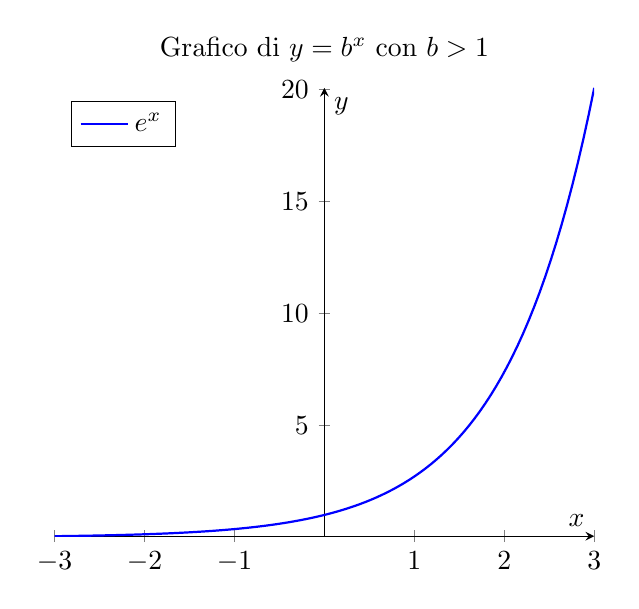
\begin{tikzpicture}
\begin{axis}[
    axis lines=middle,
    xlabel=$x$,
    ylabel=$y$,
    title={Grafico di $y = b^x$ con $b>1$},
    domain=-3:3,
    samples=100,
    legend pos=north west
]
\addplot[blue, thick] {exp(x)};
\legend{$e^x$}
\end{axis}
\end{tikzpicture}
\caption{Esempio di funzione esponenziale con base $b=e > 1$.}
\end{figure}

\begin{figure}[!htbp]
\centering
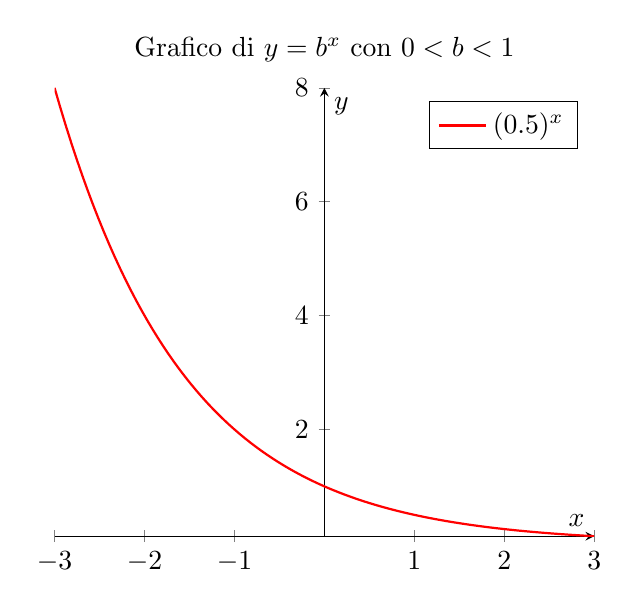
\begin{tikzpicture}
\begin{axis}[
    axis lines=middle,
    xlabel=$x$,
    ylabel=$y$,
    title={Grafico di $y = b^x$ con $0<b<1$},
    domain=-3:3,
    samples=100,
    legend pos=north east
]
\addplot[red, thick] {0.5^x};
\legend{$(0.5)^x$}
\end{axis}
\end{tikzpicture}
\caption{Esempio di funzione esponenziale con base $b=0.5 < 1$.}
\end{figure}
